\documentclass[twocolumn]{article}

\usepackage[margin=0.70in]{geometry}
\usepackage{lipsum,mwe,abstract,hyperref}
\usepackage[english]{babel} 
\usepackage{fancyhdr}

\hypersetup{hidelinks}
\setlength\parindent{0pt} 

\usepackage{amsmath,amsfonts,amsthm}
\usepackage{wrapfig}
\usepackage{graphicx}
\usepackage{float}
\usepackage{subcaption}
\usepackage{comment}
\usepackage{enumitem}
\usepackage{cuted}
\usepackage{sectsty}

\allsectionsfont{\normalfont \normalsize \scshape} 

\renewenvironment{abstract}
 {\small
  \begin{center}
  \bfseries \abstractname\vspace{-.5em}\vspace{0pt}
  \end{center}
  \list{}{
    \setlength{\leftmargin}{0mm}
    \setlength{\rightmargin}{\leftmargin}
  }
  \item\relax}
 {\endlist}
 
\makeatletter
\renewcommand{\maketitle}{\bgroup\setlength{\parindent}{0pt}
\begin{flushleft}
  \textbf{\@title}
  \@author \\ 
  \@date
\end{flushleft}\egroup
}
\makeatother

\title{\Large Title of Whitepaper \\
[10pt]
}

\date{\today}
\author{John Doe}

\begin{document}

\twocolumn[\maketitle]

\begin{abstract}
    \lipsum[1]
\end{abstract}

\rule{\linewidth}{0.5pt}

\section{Introduction}
\lipsum[2]

\section{Section Title}
\lipsum[1-2]

\section{Section Title}

\lipsum[1]

\begin{figure}[H]
    \centering
    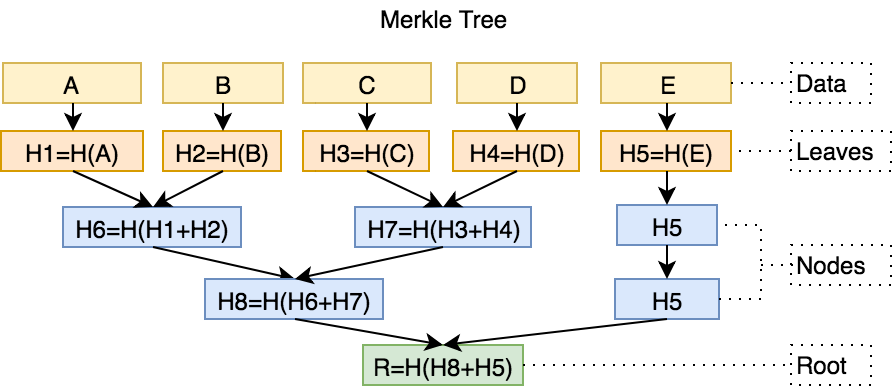
\includegraphics[width=0.425\textwidth]{merkle_tree.png}
    \caption{Merkle Hash-Tree \cite{merkle_hash_tree_graphic}}
\end{figure}

\lipsum[2]

\subsection{Subsection Title}

\lipsum[1]

\subsection{Subsection Title}

\lipsum[1]

\section{Conclusion}

\lipsum [4-5]

\begin{thebibliography}{}
    \bibitem{merkle_hash_tree_graphic}{\url{https://github.com/miguelmota/merkletreejs}}
\end{thebibliography}

\end{document}
